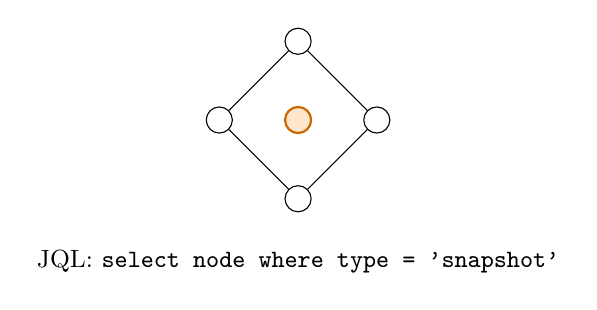
\begin{tikzpicture}[
    rnode/.style={circle, draw=black, fill=white, minimum size=6pt},
    highlight/.style={circle, draw=orange!80!black, fill=orange!20, minimum size=8pt, thick},
    arrow/.style={->, thick}
]

\node[rnode] (A) at (0,0) {};
\node[rnode] (B) at (1,1) {};
\node[rnode] (C) at (2,0) {};
\node[rnode] (D) at (1,-1) {};

\draw (A)--(B)--(C)--(D)--(A);

\node[highlight] at (1,0) {};

\node at (1,-1.8) {\small JQL: \texttt{select node where type = 'snapshot'}};

\end{tikzpicture}